\section{High-Level Language Design}
\label{sec:high-level-language-design}

\sidefigure[0.45]{figures/Dialect definitions and a rewrite rule.pdf}
  {A rule file imports operation definitions from a dialect file.}
  {fig:dialect-rule}
  {The file my_dialect.tepl defines MyDialect with transpose and dot operations. An import arrow connects it to my_rule.tepl, which imports the dialect and defines a rewrite from dot with transpose to dot.}

\subsection{Dialects, Operations, and Rewrite Rules}
\label{sec:dialects-operations-and-rewrite-rules}
TEPL separates operation definitions from rewrite rules.
In Figure~\ref{fig:dialect-rule}, \code{my_dialect.tepl} defines
\emph{MyDialect}, which groups the \code{transpose} and \code{dot}
operations. Each operation declares its operands, result, attributes,
and semantics. Section~\ref{sec:axis-extent-and-coordinate-attributes} explains the attribute roles.

The file \code{my_rule.tepl} imports this dialect and defines a
\emph{rewrite rule} using \code{LHS => RHS}.
Each side is an s-expression of the form \code{(operation operands)},
where operands can themselves be nested expressions.
The example replaces a dot with a transposed input by a single dot.
The replacement's attributes must account for the removed transpose.

Each operation node can have its own name.
For example, \code{(d: dot X Y)} names the dot node \code{d}.
This name is used in \code{where} and \code{derive} blocks to access
the node's attributes, express conditions, and compute replacement
attributes, as explained below.

\subsection{Axis, Extent, and Coordinate Attributes}
\label{sec:axis-extent-and-coordinate-attributes}

TEPL requires a type when declaring an operation attribute and distinguishes
three roles for integer attributes: axes, extents, and coordinates
(Figure~\ref{fig:attribute-roles}). These roles describe different properties
even when their integer values coincide. This distinction allows TEPL to
target axis fields for synthesis, while extent and coordinate
attributes remain supplied.

\begin{table}[H]
\begin{minipage}[t]{0.68\linewidth}
\vspace{0pt}
\caption{Integer-attribute roles in TEPL.}
\label{tab:attribute-roles}
\small
\setlength{\tabcolsep}{4pt}
\begin{tabularx}{\linewidth}{@{}lYl@{}}\toprule
Role & Meaning & Example field\\\midrule
\code{axis} & Dimension position & Transpose \code{permutation: axis[]}\\
\code{extent} & Dimension size & Reshape \code{shape: extent[]}\\
\code{coordinate} & Position, offset, or stride & Slice \code{starts: coordinate[]}\\\bottomrule
\end{tabularx}
\end{minipage}\hfill
\begin{minipage}[t]{0.3\linewidth}
\vspace{0pt}
\centering
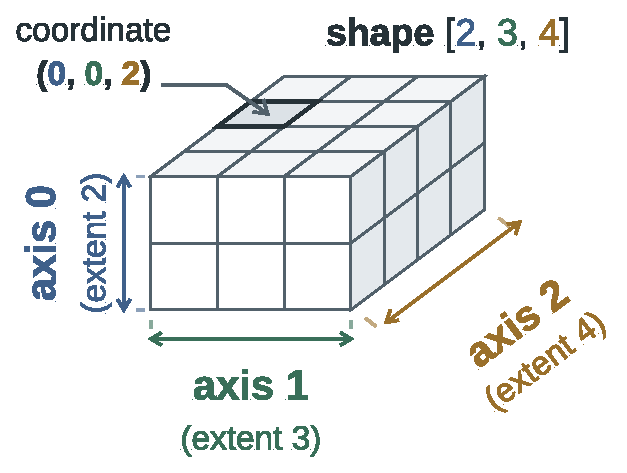
\includegraphics[width=\linewidth]{figures/Axis, extent, and coordinate.pdf}
\captionsetup{type=figure}
\caption{Axis, extent, and coordinate in a tensor of shape $(2,3,4)$.}
\label{fig:attribute-roles}
\Description{A three-dimensional tensor with vertical axis 0 of extent 2, horizontal axis 1 of extent 3, and depth axis 2 of extent 4. The highlighted element has coordinate (0, 0, 2). Matching colors associate each axis with its shape and coordinate entries.}
\end{minipage}
\end{table}


\sidefigure[0.5]{figures/Attribute Binding and Derivation.pdf}{Captured operation attributes can be read in \code{where} and \code{derive} blocks. The \code{derive} block explicitly defines RHS attribute transformation logic using these captured attributes.}{fig:attribute-binding}{An input graph with transpose and dot is replaced by a dot. Colored descriptor
bindings connect the rule to a table with two captured rows and one derived row.}

\subsection{Conditions with \texorpdfstring{\code{where}}{where}}
\label{sec:conditions-with-where}

A \code{where} block adds conditions that a match must satisfy before
a rule can apply. Users can combine conditions with \code{&&} and
\code{||} to restrict axis lists, dimension sizes, or backend requirements.
Omitting the block adds no user-defined restriction.


\subsection{Attribute Binding and Explicit Derivation}
\label{sec:attribute-binding-and-explicit-derivation}

When a rule matches, TEPL captures the attributes of its LHS operations.
A named node exposes these attributes through \code{node.attrs}.

Users can compute RHS attributes in a \code{derive} block and assign
them to a named node's \code{attrs} property
(Figure~\ref{fig:attribute-binding}).
When no change is needed, bracket notation reuses an existing attribute
record: \code{(dot[d.attrs] A B)} gives the RHS dot the attributes of
\code{d}. The reused attributes must be compatible with the replacement
operation, and the rewrite must still preserve the result.

\par\wrapstuffclear
\noindent\begin{minipage}{\linewidth}
For example, \code{gather} composes two captured transpose permutations:
\begin{lstlisting}[language=TEPL]
rule compose_transposes_explicit {
  (t2: transpose (t1: transpose X)) => (t3: transpose X)
  derive {
    t3.attrs = {
      permutation: gather(t1.attrs.permutation, t2.attrs.permutation)
    };
  }
}
\end{lstlisting}
\end{minipage}

\par\wrapstuffclear
% Align the subsection heading, text, and listing beside the figure.
\noindent
\begin{minipage}[t]{0.46\linewidth}
\vspace{0pt}
\subsection{Automatic Attribute Inference}
\label{sec:automatic-attribute-inference}
When RHS axis fields are omitted and no derivation is provided for them, TEPL asks the
compiler to infer their transformation logic. The same transpose rewrite
can therefore be written without a \code{derive} block:

\begin{lstlisting}[language=TEPL]
rule compose_transposes_auto {
  (transpose (transpose X))
  => (transpose X)
}
\end{lstlisting}

The compiler infers the explicit permutation transformation above once
(Figure~\ref{fig:introducing-auto}). When an operation has both axis and
non-axis attributes, users supply the non-axis fields explicitly in a
\code{derive} block while leaving the axis fields omitted or set to
\code{auto} for inference.

TEPL also generates a feasibility check to determine whether it can
construct valid RHS attributes. A rule applies only when both the
written conditions and this check pass.
Section~\ref{sec:synthesis-and-execution-contract} explains how these checks govern rule application.

\end{minipage}\hfill
\begin{minipage}[t]{0.5\linewidth}
\vspace{0pt}
\centering
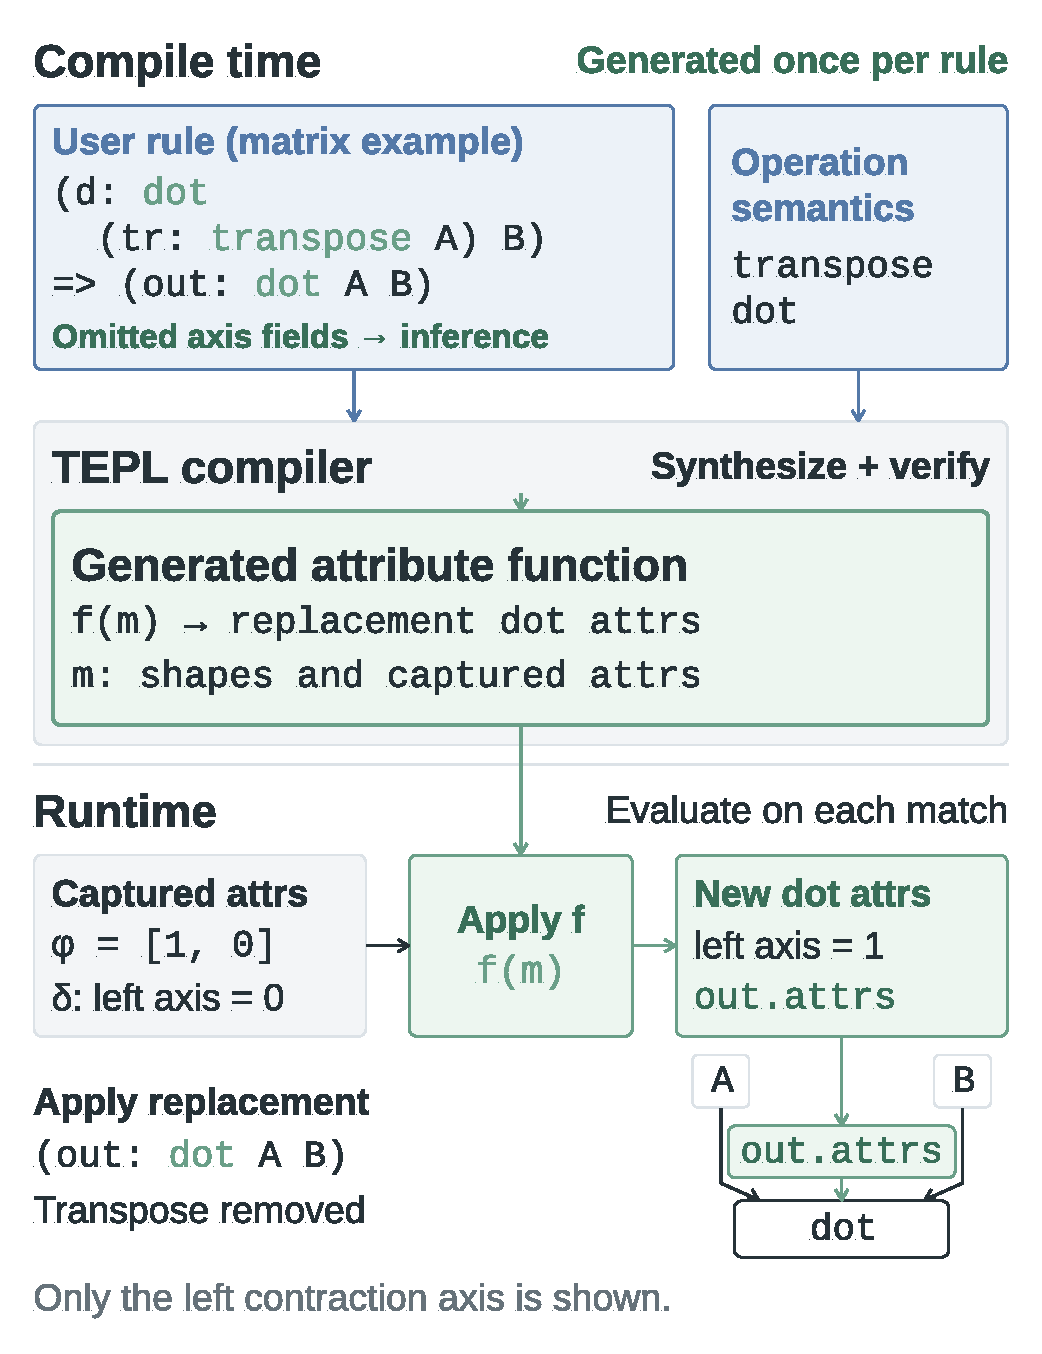
\includegraphics[width=\linewidth]{figures/Automatic Attribute Inference.pdf}
\captionsetup{type=figure,hypcap=false}
\caption{Omitted RHS axis fields trigger inference of a reusable feasibility check and attribute function at compile time.}
\label{fig:introducing-auto}
\Description{A vertical flow separates the user rule and operation semantics, compiler synthesis and verification, and runtime application of the generated function.}
\end{minipage}
\par
\FloatBarrier
